\documentclass[a4paper,12pt]{article}
\usepackage{xcolor}
\usepackage{amsmath,amsfonts,amssymb}
\usepackage{geometry}
\usepackage{fancyhdr}
\usepackage{graphicx}
\usepackage{titlesec}
\usepackage{tikz}
\usepackage{booktabs}
\usepackage{array}
\usetikzlibrary{shadows}
\usepackage{tcolorbox}
\usepackage{float}
\usepackage{lipsum}
\usepackage{mdframed}
\usepackage{pagecolor}
\usepackage{mathpazo}   % Palatino font (serif)
\usepackage{microtype}  % Better typography
\usepackage{url}

\setlength{\parindent}{0pt}

% Page background color
\pagecolor{gray!10!white}

% Geometry settings
\geometry{margin=0.5in}
\pagestyle{fancy}
\fancyhf{}

% Fancy header and footer
\fancyhead[C]{\textbf{\color{blue!80}The Evil Eye}}
% \fancyhead[R]{\color{blue!80}Saksham Rathi}
\fancyfoot[C]{\thepage}

% Custom Section Color and Format with Sans-serif font
\titleformat{\section}
{\sffamily\color{purple!90!black}\normalfont\Large\bfseries}
{\thesection}{1em}{}

% Custom subsection format
\titleformat{\subsection}
{\sffamily\color{cyan!80!black}\normalfont\large\bfseries}
{\thesubsection}{1em}{}

% Stylish Title with TikZ (Enhanced with gradient)
\newcommand{\cooltitle}[1]{%
\begin{tikzpicture}
\node[fill=blue!20,rounded corners=10pt,inner sep=12pt, drop shadow, top color=blue!50, bottom color=blue!30] (box)
{\Huge \bfseries \color{black} #1};
\end{tikzpicture}
}
\usepackage{float} % Add this package

\newenvironment{solution}[2][]{%
\begin{mdframed}[linecolor=blue!70!black, linewidth=2pt, roundcorner=10pt, backgroundcolor=yellow!10!white, skipabove=12pt, skipbelow=12pt]%
	\textbf{\large #2}
	\par\noindent\rule{\textwidth}{0.4pt}
}{
\end{mdframed}
}

% Document title
\title{\cooltitle{CS790 Assignment 2} \\
\LARGE \textbf{The Evil Eye} \\
Report}
\author{{\bf Kavya Gupta (22B1053)} \\
\small Department of Computer Science, \\
Indian Institute of Technology Bombay \\}
\date{}

\begin{document}
\maketitle

\begin{solution}{Approach}
I observed that the Vanilla TOR uses (18) specific cipher suites (See Figure \ref{cipher-suites}). So, for any TLS Client Hello, I get the cipher suite list and match it with these 18. If they match exactly, I deem the destination IP address as a TOR guard IP (and add it to a list). After this, any TCP packet, with (source/destination) IP same as any present in the list, is marked as a TOR packet.
\begin{figure}[H]
    \centering
    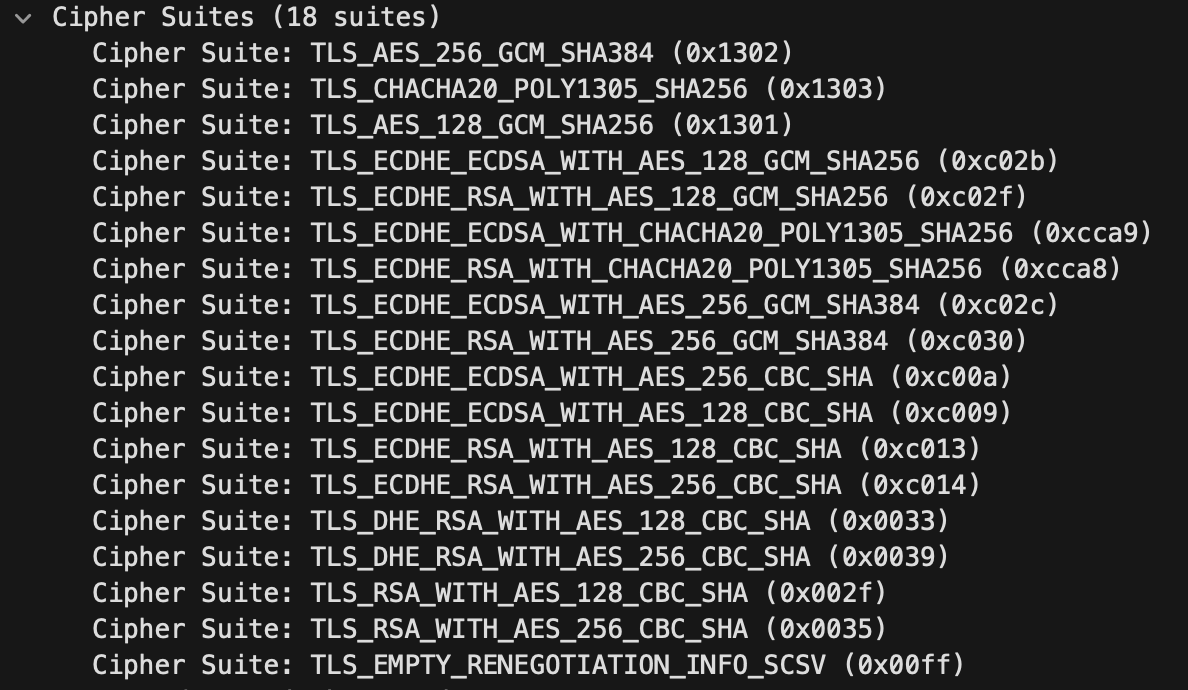
\includegraphics[width=0.5\textwidth]{cipher-suites.png}
    \caption{Vanilla TOR Cipher Suites}\label{cipher-suites}
\end{figure}
\textbf{Note:} I have made an assumption that a TOR IP remains a TOR IP (atleast for the time the Wireshark capture is recorded).
\end{solution}

\begin{solution}{Implementation}
\begin{itemize}
    \item Programmed in Lua.
    \item Wireshark has this class called \texttt{Dissector} which is used to decode (dissect) packets. They extract the fields, call upper layer dissectors (if needed) and present the extracted info as part of a `tree' in the packet info. So I had to create my own dissector function that will extract necessary information and deem a packet as TOR as told in the above approach.
    \item To do that, I had to first create a \texttt{Proto} (protocol) object and then wrote the dissector. In this function, I call the dissector of TCP first (which was acquired using \texttt{DissectorTable.get()}). This will chop down the packet and make fields (of TCP and TLS (if present)) available.
    \item Then I check if the packet is a TLS Client Hello packet by checking if \texttt{tls.handshake.type} is 1. I acquired its value using the class \texttt{Field}. Using \texttt{Field.new(<fieldname>)}, I can get the value of any field in the packet. Value of \texttt{tls.handshake.ciphersuites} field gives the list of cipher suites used in the packet and I check if it matches with the TOR cipher suites. If it does, I add the destination IP address (got using \texttt{Field.new("ip.dst")}) to a list (of TOR IPs).
    \item Then in the function, I extract the source IP and destionation IP addresses and check if any of them is present in the list. If yes, I mark the packet as a TOR packet (to show this I just append \texttt{" (Tor!)"} to the Protocol column, see figure \ref{tor-display}).
    \item Finally this dissector has to be added to the \texttt{DissectorTable}. Using \texttt{.add()}, I coded that if the protocol field of the IP header is 6 (which is TCP), then call my dissector function.
\end{itemize}
\begin{figure}[H]
    \centering
    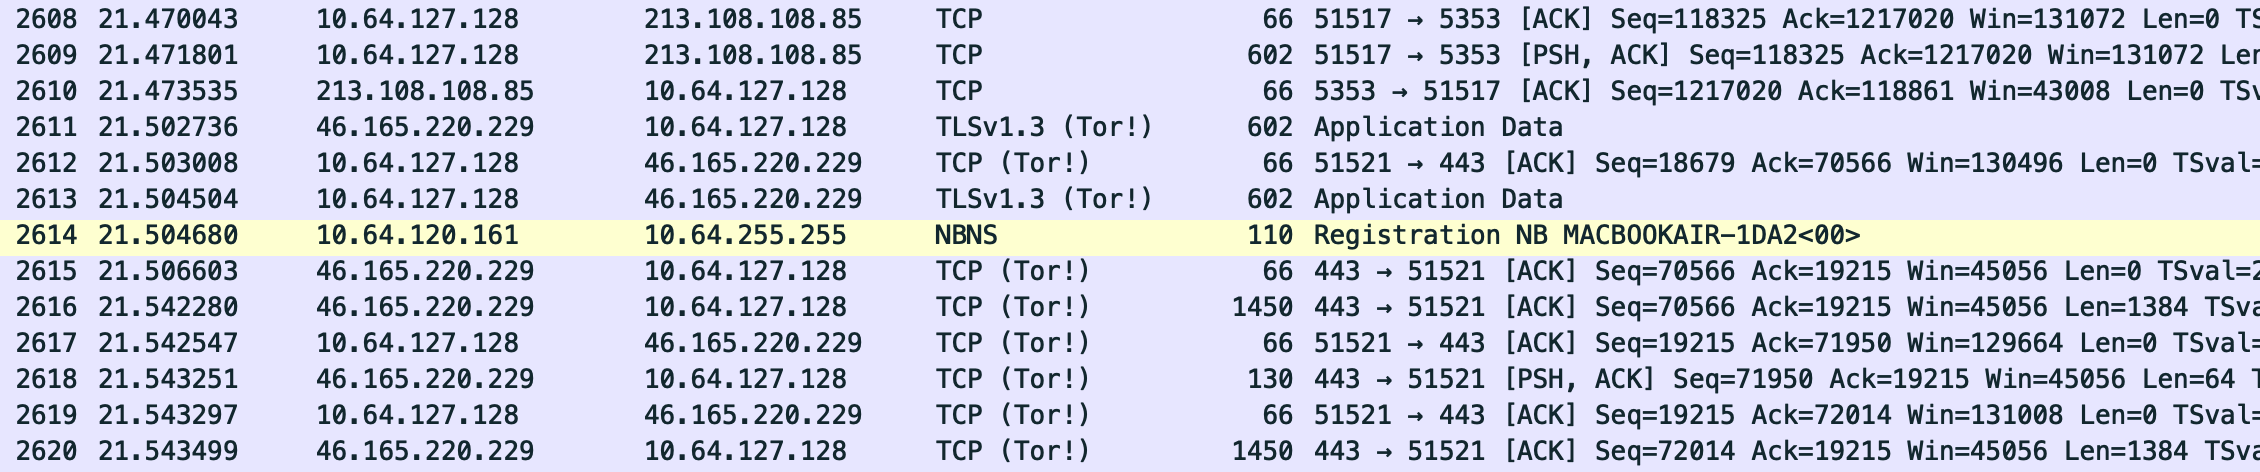
\includegraphics[width=0.75\textwidth]{tor-display.png}
    \caption{Tor display in Wireshark}\label{tor-display}
\end{figure}
\end{solution}

\begin{solution}{Files Submitted}
\begin{itemize}
    \item \texttt{tor\_detector.lua}
    \item \texttt{sample.pcap}
    \item \texttt{report.pdf}
    \item \texttt{README.txt}
\end{itemize}
\end{solution}

\begin{solution}{References}
\begin{itemize}
    \item Little help from ChatGPT, Google.
    \item {\small \url{https://www.wireshark.org/docs/wsdg_html_chunked/wsluarm_modules.html}}: Wireshark Lua API Reference Manual
\end{itemize}
\end{solution}

\end{document}